% LaTeX path to the root directory of the current project, from the directory in which this file resides
% and path to econtexPaths which defines the rest of the paths like \FigDir
\providecommand{\econtexRoot}{}\renewcommand{\econtexRoot}{.}
\providecommand{\econtexPaths}{}\renewcommand{\econtexPaths}{\econtexRoot/Resources/econtexPaths}
% The \commands below are required to allow sharing of the same base code via Github between TeXLive on a local machine and Overleaf (which is a proxy for "a standard distribution of LaTeX").  This is an ugly solution to the requirement that custom LaTeX packages be accessible, and that Overleaf prohibits symbolic links

\providecommand{\econtex}{\econtexRoot/Resources/texmf-local/tex/latex/econtex}
\providecommand{\pdfsuppressruntime}{\econtexRoot/Resources/texmf-local/tex/latex/pdfsuppressruntime}
\providecommand{\econark}{/Volumes/Sync/GitHub/llorracc/SolvingMicroDSOPs/SolvingMicroDSOPs-Latest/.resources/texmf-local/tex/latex/local-econark}
\providecommand{\econtexSetup}{\econtexRoot/Resources/texmf-local/tex/latex/econtexSetup}
\providecommand{\econtexShortcuts}{\econtexRoot/Resources/texmf-local/tex/latex/econtexShortcuts}
\providecommand{\econtexBibMake}{\econtexRoot/Resources/texmf-local/tex/latex/econtexBibMake}
\providecommand{\econtexBibStyle}{\econtexRoot/Resources/texmf-local/bibtex/bst/econtex}
\providecommand{\econtexBib}{economics}
\providecommand{\economics}{\econtexRoot/Resources/texmf-local/bibtex/bib/economics}
\providecommand{\notes}{\econtexRoot/Resources/texmf-local/tex/latex/handout}
\providecommand{\handoutSetup}{\econtexRoot/Resources/texmf-local/tex/latex/handoutSetup}
\providecommand{\handoutShortcuts}{\econtexRoot/Resources/texmf-local/tex/latex/handoutShortcuts}
\providecommand{\handoutBibMake}{\econtexRoot/Resources/texmf-local/tex/latex/handoutBibMake}
\providecommand{\handoutBibStyle}{\econtexRoot/Resources/texmf-local/bibtex/bst/handout}

\providecommand{\FigDir}{\econtexRoot/Figures}
\providecommand{\CodeDir}{\econtexRoot/Code}
\providecommand{\DataDir}{\econtexRoot/Data}
\providecommand{\SlideDir}{\econtexRoot/Slides}
\providecommand{\TableDir}{\econtexRoot/Tables}
\providecommand{\ApndxDir}{\econtexRoot/Appendices}

\providecommand{\ResourcesDir}{\econtexRoot/Resources}
\providecommand{\rootFromOut}{..} % APFach back to root directory from output-directory
\providecommand{\LaTeXGenerated}{\econtexRoot/LaTeX} % Put generated files in subdirectory
\providecommand{\econtexPaths}{\econtexRoot/Resources/econtexPaths}
\providecommand{\LaTeXInputs}{\econtexRoot/Resources/LaTeXInputs}
\providecommand{\LtxDir}{}
\providecommand{\EqDir}{Equations} % Put generated files in subdirectory

\documentclass[\econtexRoot/BufferStockTheory]{subfiles}
% LaTeX path to the root directory of the current project, from the directory in which this file resides
% and path to econtexPaths which defines the rest of the paths like \FigDir
\providecommand{\econtexRoot}{}\renewcommand{\econtexRoot}{.}
\providecommand{\econtexPaths}{}\renewcommand{\econtexPaths}{\econtexRoot/Resources/econtexPaths}
% The \commands below are required to allow sharing of the same base code via Github between TeXLive on a local machine and Overleaf (which is a proxy for "a standard distribution of LaTeX").  This is an ugly solution to the requirement that custom LaTeX packages be accessible, and that Overleaf prohibits symbolic links

\providecommand{\econtex}{\econtexRoot/Resources/texmf-local/tex/latex/econtex}
\providecommand{\pdfsuppressruntime}{\econtexRoot/Resources/texmf-local/tex/latex/pdfsuppressruntime}
\providecommand{\econark}{/Volumes/Sync/GitHub/llorracc/SolvingMicroDSOPs/SolvingMicroDSOPs-Latest/.resources/texmf-local/tex/latex/local-econark}
\providecommand{\econtexSetup}{\econtexRoot/Resources/texmf-local/tex/latex/econtexSetup}
\providecommand{\econtexShortcuts}{\econtexRoot/Resources/texmf-local/tex/latex/econtexShortcuts}
\providecommand{\econtexBibMake}{\econtexRoot/Resources/texmf-local/tex/latex/econtexBibMake}
\providecommand{\econtexBibStyle}{\econtexRoot/Resources/texmf-local/bibtex/bst/econtex}
\providecommand{\econtexBib}{economics}
\providecommand{\economics}{\econtexRoot/Resources/texmf-local/bibtex/bib/economics}
\providecommand{\notes}{\econtexRoot/Resources/texmf-local/tex/latex/handout}
\providecommand{\handoutSetup}{\econtexRoot/Resources/texmf-local/tex/latex/handoutSetup}
\providecommand{\handoutShortcuts}{\econtexRoot/Resources/texmf-local/tex/latex/handoutShortcuts}
\providecommand{\handoutBibMake}{\econtexRoot/Resources/texmf-local/tex/latex/handoutBibMake}
\providecommand{\handoutBibStyle}{\econtexRoot/Resources/texmf-local/bibtex/bst/handout}

\providecommand{\FigDir}{\econtexRoot/Figures}
\providecommand{\CodeDir}{\econtexRoot/Code}
\providecommand{\DataDir}{\econtexRoot/Data}
\providecommand{\SlideDir}{\econtexRoot/Slides}
\providecommand{\TableDir}{\econtexRoot/Tables}
\providecommand{\ApndxDir}{\econtexRoot/Appendices}

\providecommand{\ResourcesDir}{\econtexRoot/Resources}
\providecommand{\rootFromOut}{..} % APFach back to root directory from output-directory
\providecommand{\LaTeXGenerated}{\econtexRoot/LaTeX} % Put generated files in subdirectory
\providecommand{\econtexPaths}{\econtexRoot/Resources/econtexPaths}
\providecommand{\LaTeXInputs}{\econtexRoot/Resources/LaTeXInputs}
\providecommand{\LtxDir}{}
\providecommand{\EqDir}{Equations} % Put generated files in subdirectory

\onlyinsubfile{% https://tex.stackexchange.com/questions/463699/proper-reference-numbers-with-subfiles
    \csname @ifpackageloaded\endcsname{xr-hyper}{%
      \externaldocument{BufferStockTheory}% xr-hyper in use; optional argument for url of main.pdf for hyperlinks
    }{%
      \externaldocument{BufferStockTheory}% xr in use
    }%
    \renewcommand\labelprefix{}%
    % Initialize the counters via the labels belonging to the main document:
}


\onlyinsubfile{\externaldocument{\LaTeXGenerated/BufferStockTheory}}

\begin{document}

;;; -*- coding: utf-8; -*-
      \node (pffvafNEQpfgicPfhwc) [xshift=4cm,yshift=-1.5cm]{$\neq$};
      \node (pffvafNEQricPcancelfhwc) [xshift=1.5cm,yshift=-3.8cm]{$\neq$};
      \node (thorn) {$\Pat$};
      \node (gamma) [right of = thorn] {$\PGro$};
      \node (rfree) [below of = thorn]{$\mathsf{\Rfree}$};
%      \node (pffvacFac) [right of = rfree] {$\underbrace{\Rfree^{1/\CRRA}\PGro^{1 - 1/\CRRA}}_{\equiv \PGro} $}; % \left(\equiv (\Rfree \PGro)^{1/\CRRA}\PGro\right)
      \node (pffvacFac) [right of = rfree] {$\Rfree^{1/\CRRA}\PGro^{1 - 1/\CRRA}$}; % \left(\equiv (\Rfree \PGro)^{1/\CRRA}\PGro\right)
      \draw[->] (thorn) to node {${\GICRaw}$} (gamma);
      \draw[->] (thorn) to node [swap] [rotate=-90,yshift=-0.3cm,xshift=+0.2cm]{${\RIC}$} (rfree);
      \draw[->] (thorn) to node [swap] [rotate=-45,xshift=0.5cm,yshift=+0.4cm] {$\PFFVAC$} (pffvacFac);
      \draw[->] (gamma) to node [rotate=-90,xshift=-0.7cm,yshift=+0.3cm]{${\FHWC}$} (pffvacFac);
      \draw[<-] (pffvacFac) to node{\cncl{\FHWC}} (rfree); 

 % Store the tex for standalone compilation
 \ifthenelse{\boolean{Web}}{
\begin{figure}[tbp] % Web
\centerline{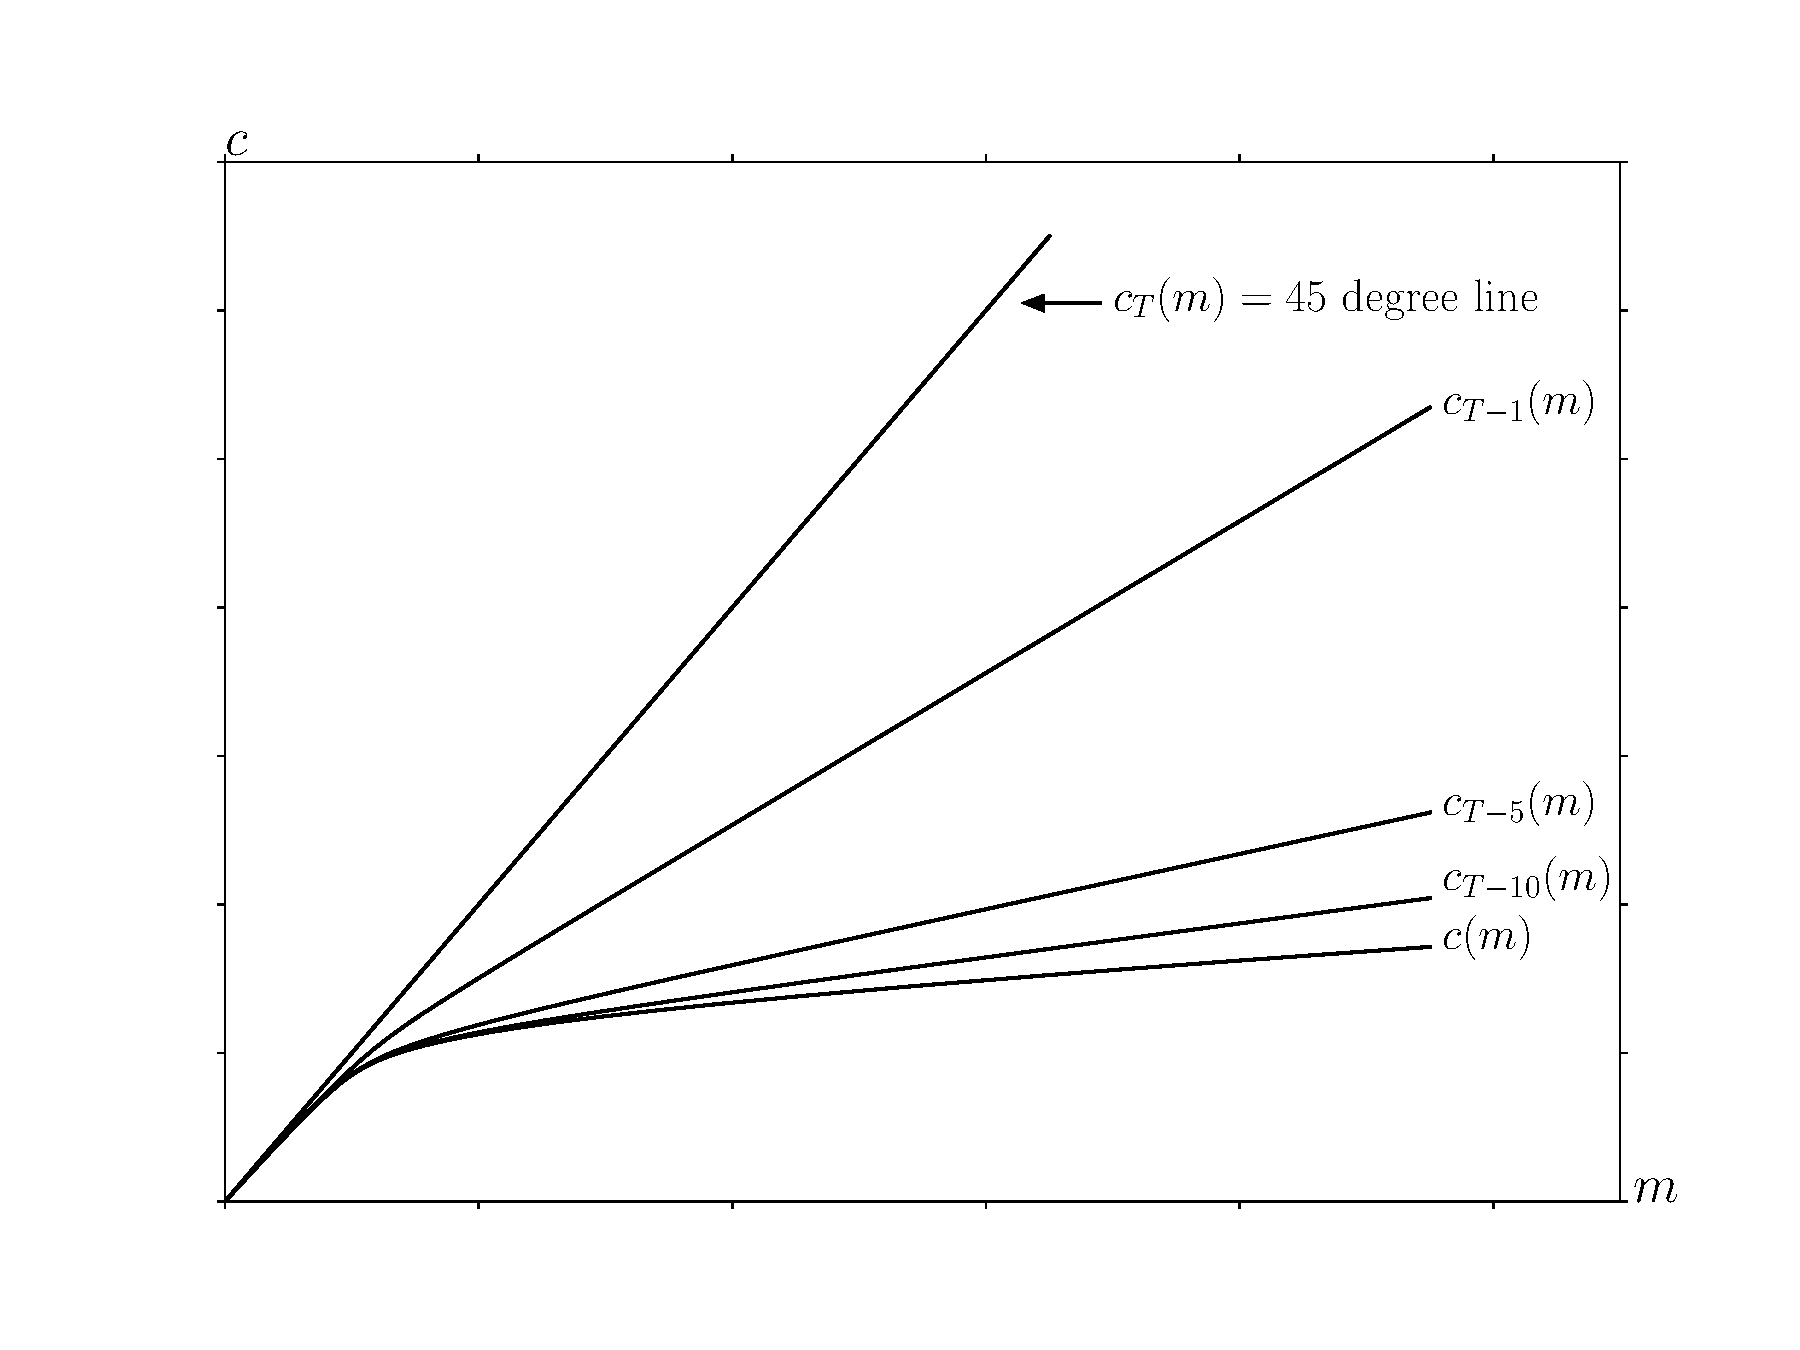
\includegraphics[width=0.7\linewidth]{\FigDir/cFuncsConverge}} % Web 
\caption{Convergence of the Consumption Rules} % Web 
\label{fig:cFuncsConverge} % Web 
\end{figure} % Web
}{ % Web - no
\begin{figure}[tbp]
\centerline{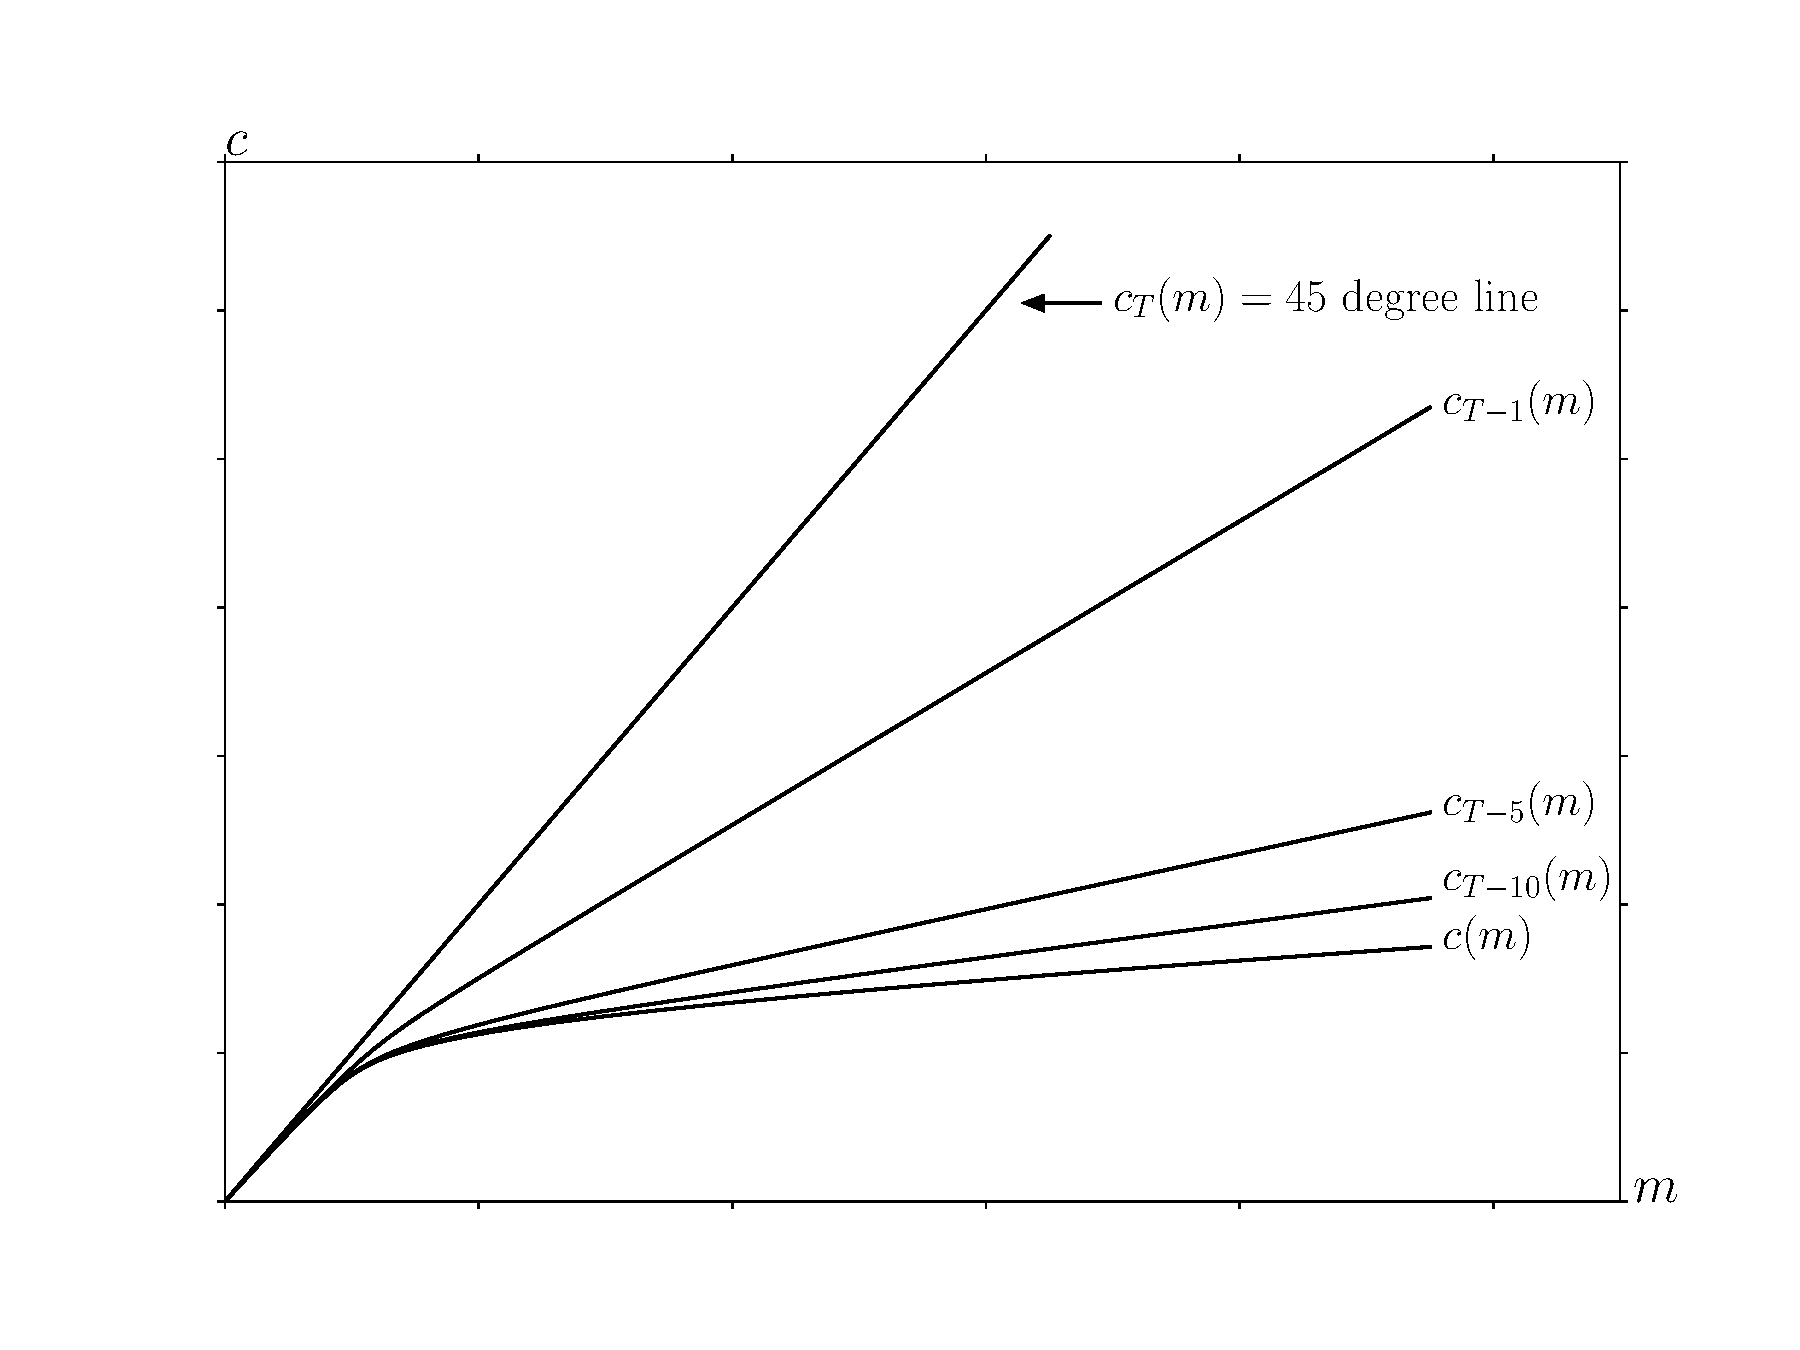
\includegraphics[width=5.25in]{\FigDir/cFuncsConverge}}
\caption{Convergence of the Consumption Rules}
\label{fig:cFuncsConverge}
\end{figure}
} % Web - no

\begin{figure}[ht]
  \centerline{
    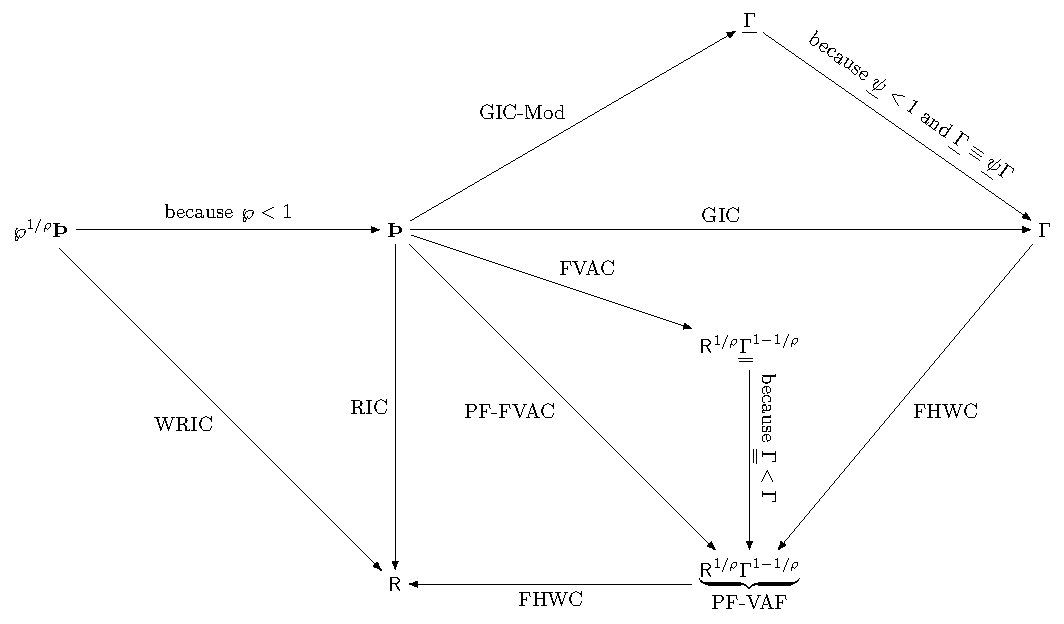
\includegraphics[width=6.0in]{\FigDir/Inequalities}
  }
  \caption{Relation of All Inequality Conditions} \label{fig:Inequalities}
\centerline{See Table~\ref{table:Calibration} for Numerical Values of Nodes Under Baseline Parameters}
\end{figure}

\hypertarget{FVACnotGIC}{}
\begin{figure}[tbp]
\centerline{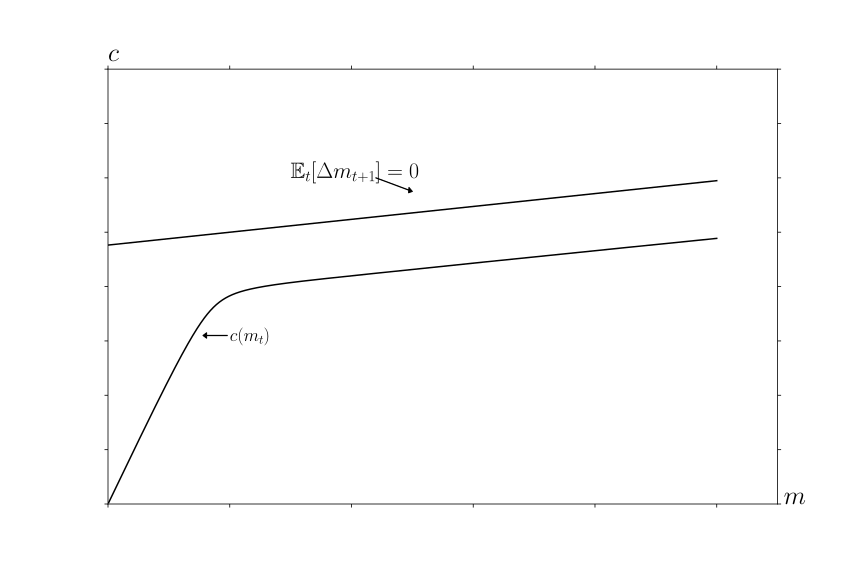
\includegraphics[width=6in]{Figures/FVACnotGIC}}
\caption{Example Solution under \{{FVAC},\cncl{GIC-Mod}\}}
\label{fig:FVACnotGIC}
\end{figure}

% Could not get fonts to work right for svg version of this figure for web; so use png
\ifthenelse{\boolean{Web}}{
\begin{figure}[tbp] % Web
\centerline{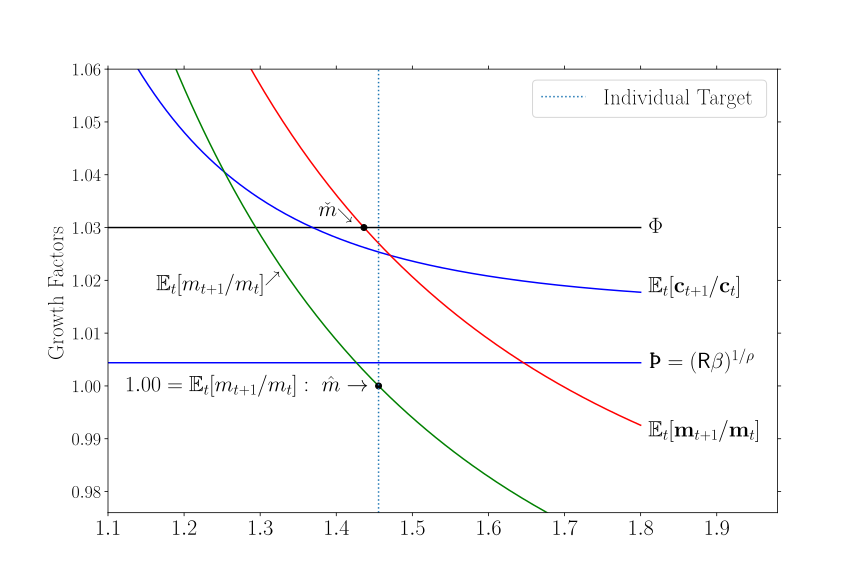
\includegraphics[width=0.8\linewidth]{\FigDir/cNrmTargetFig}} % Web 
\caption{`Stable' $\mNrm$ Values and Expected Growth Rates} % Web 
\label{fig:cNrmTargetFig} % Web
\end{figure} % Web
}{ % Web - no
\begin{figure}[tbp]
\centerline{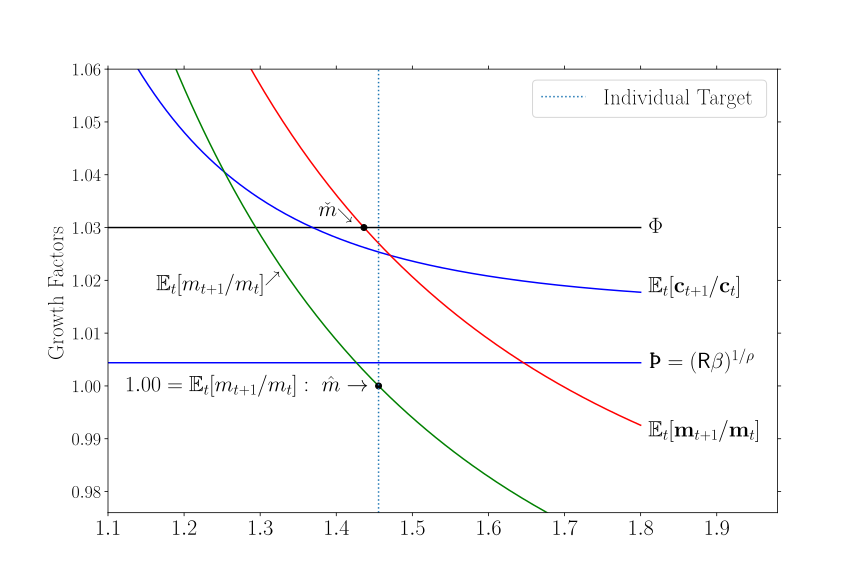
\includegraphics[width=0.8\textwidth]{\FigDir/cNrmTargetFig}}
\caption{Buffer Stock Target and Pseudo-Target}
\label{fig:cNrmTargetFig}
\end{figure}
} % Web

\hypertarget{MPCLimits}{}
 \ifthenelse{\boolean{Web}}{
\begin{figure} % Web
\centerline{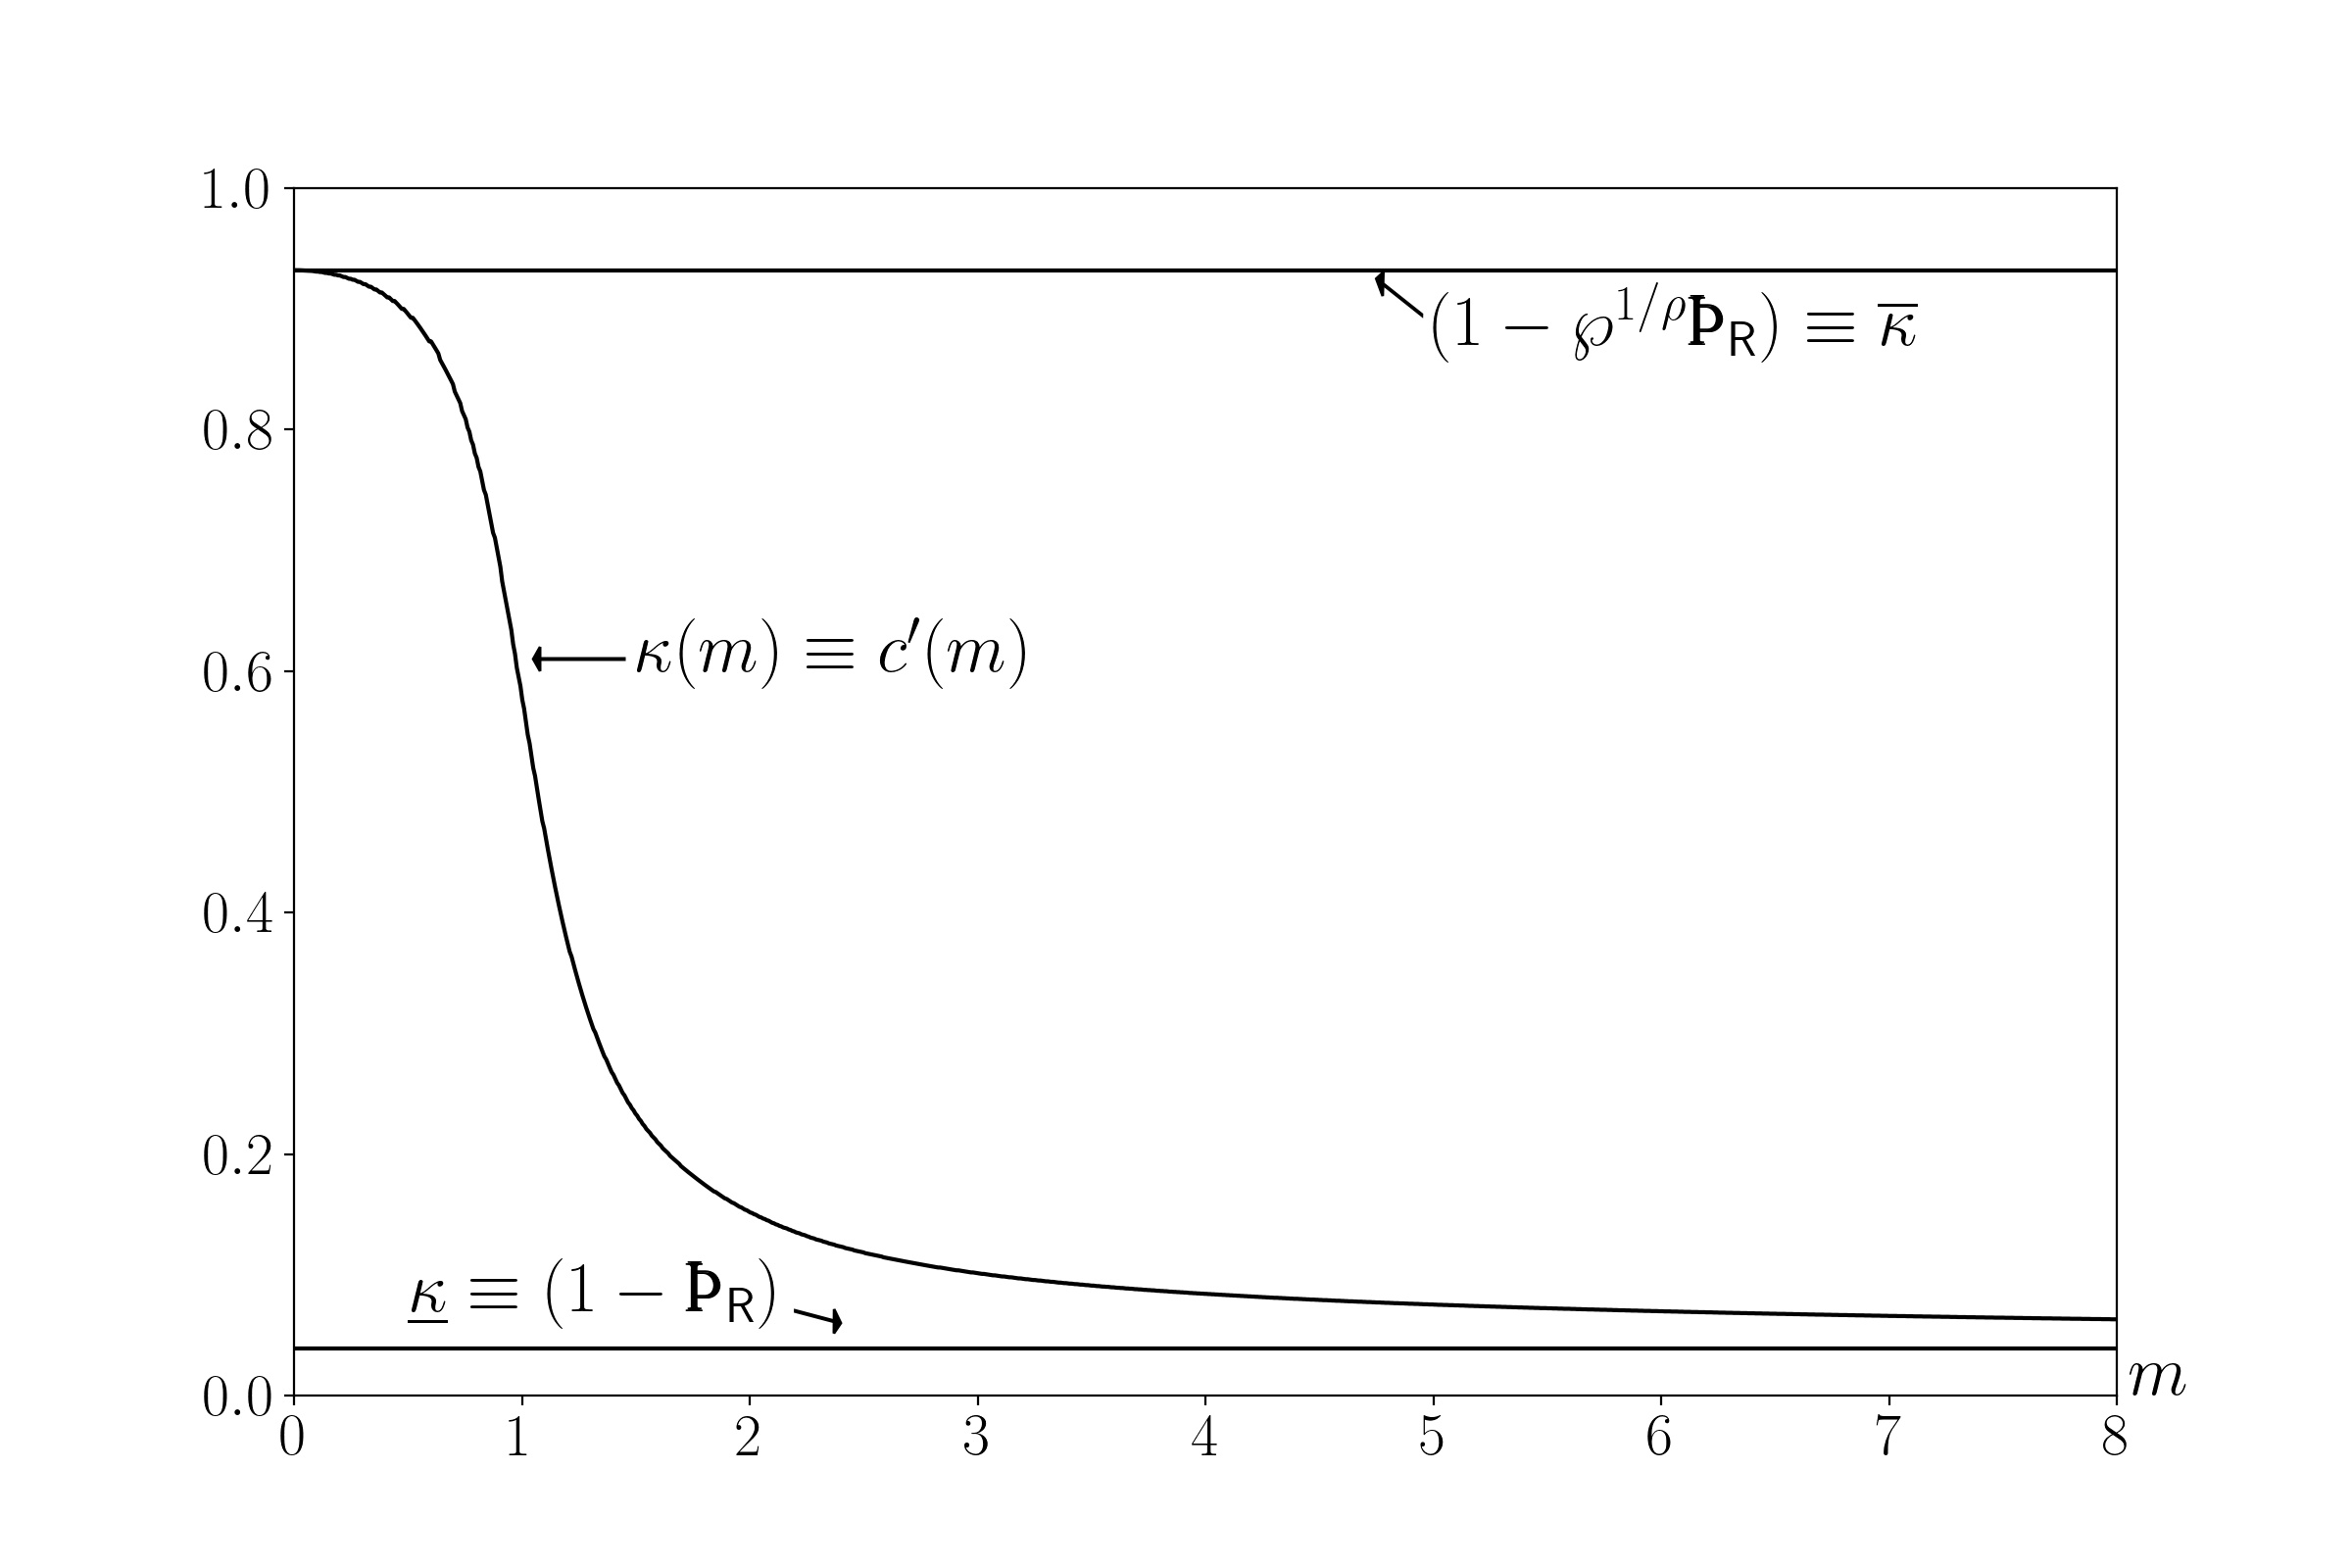
\includegraphics[width=0.8\linewidth]{\FigDir/MPCLimits}}  % Web 
\caption{Limiting MPC's} % Web 
\label{fig:mpclimits} % Web
\end{figure} % Web
}{ % Web - no
\begin{figure}
\centerline{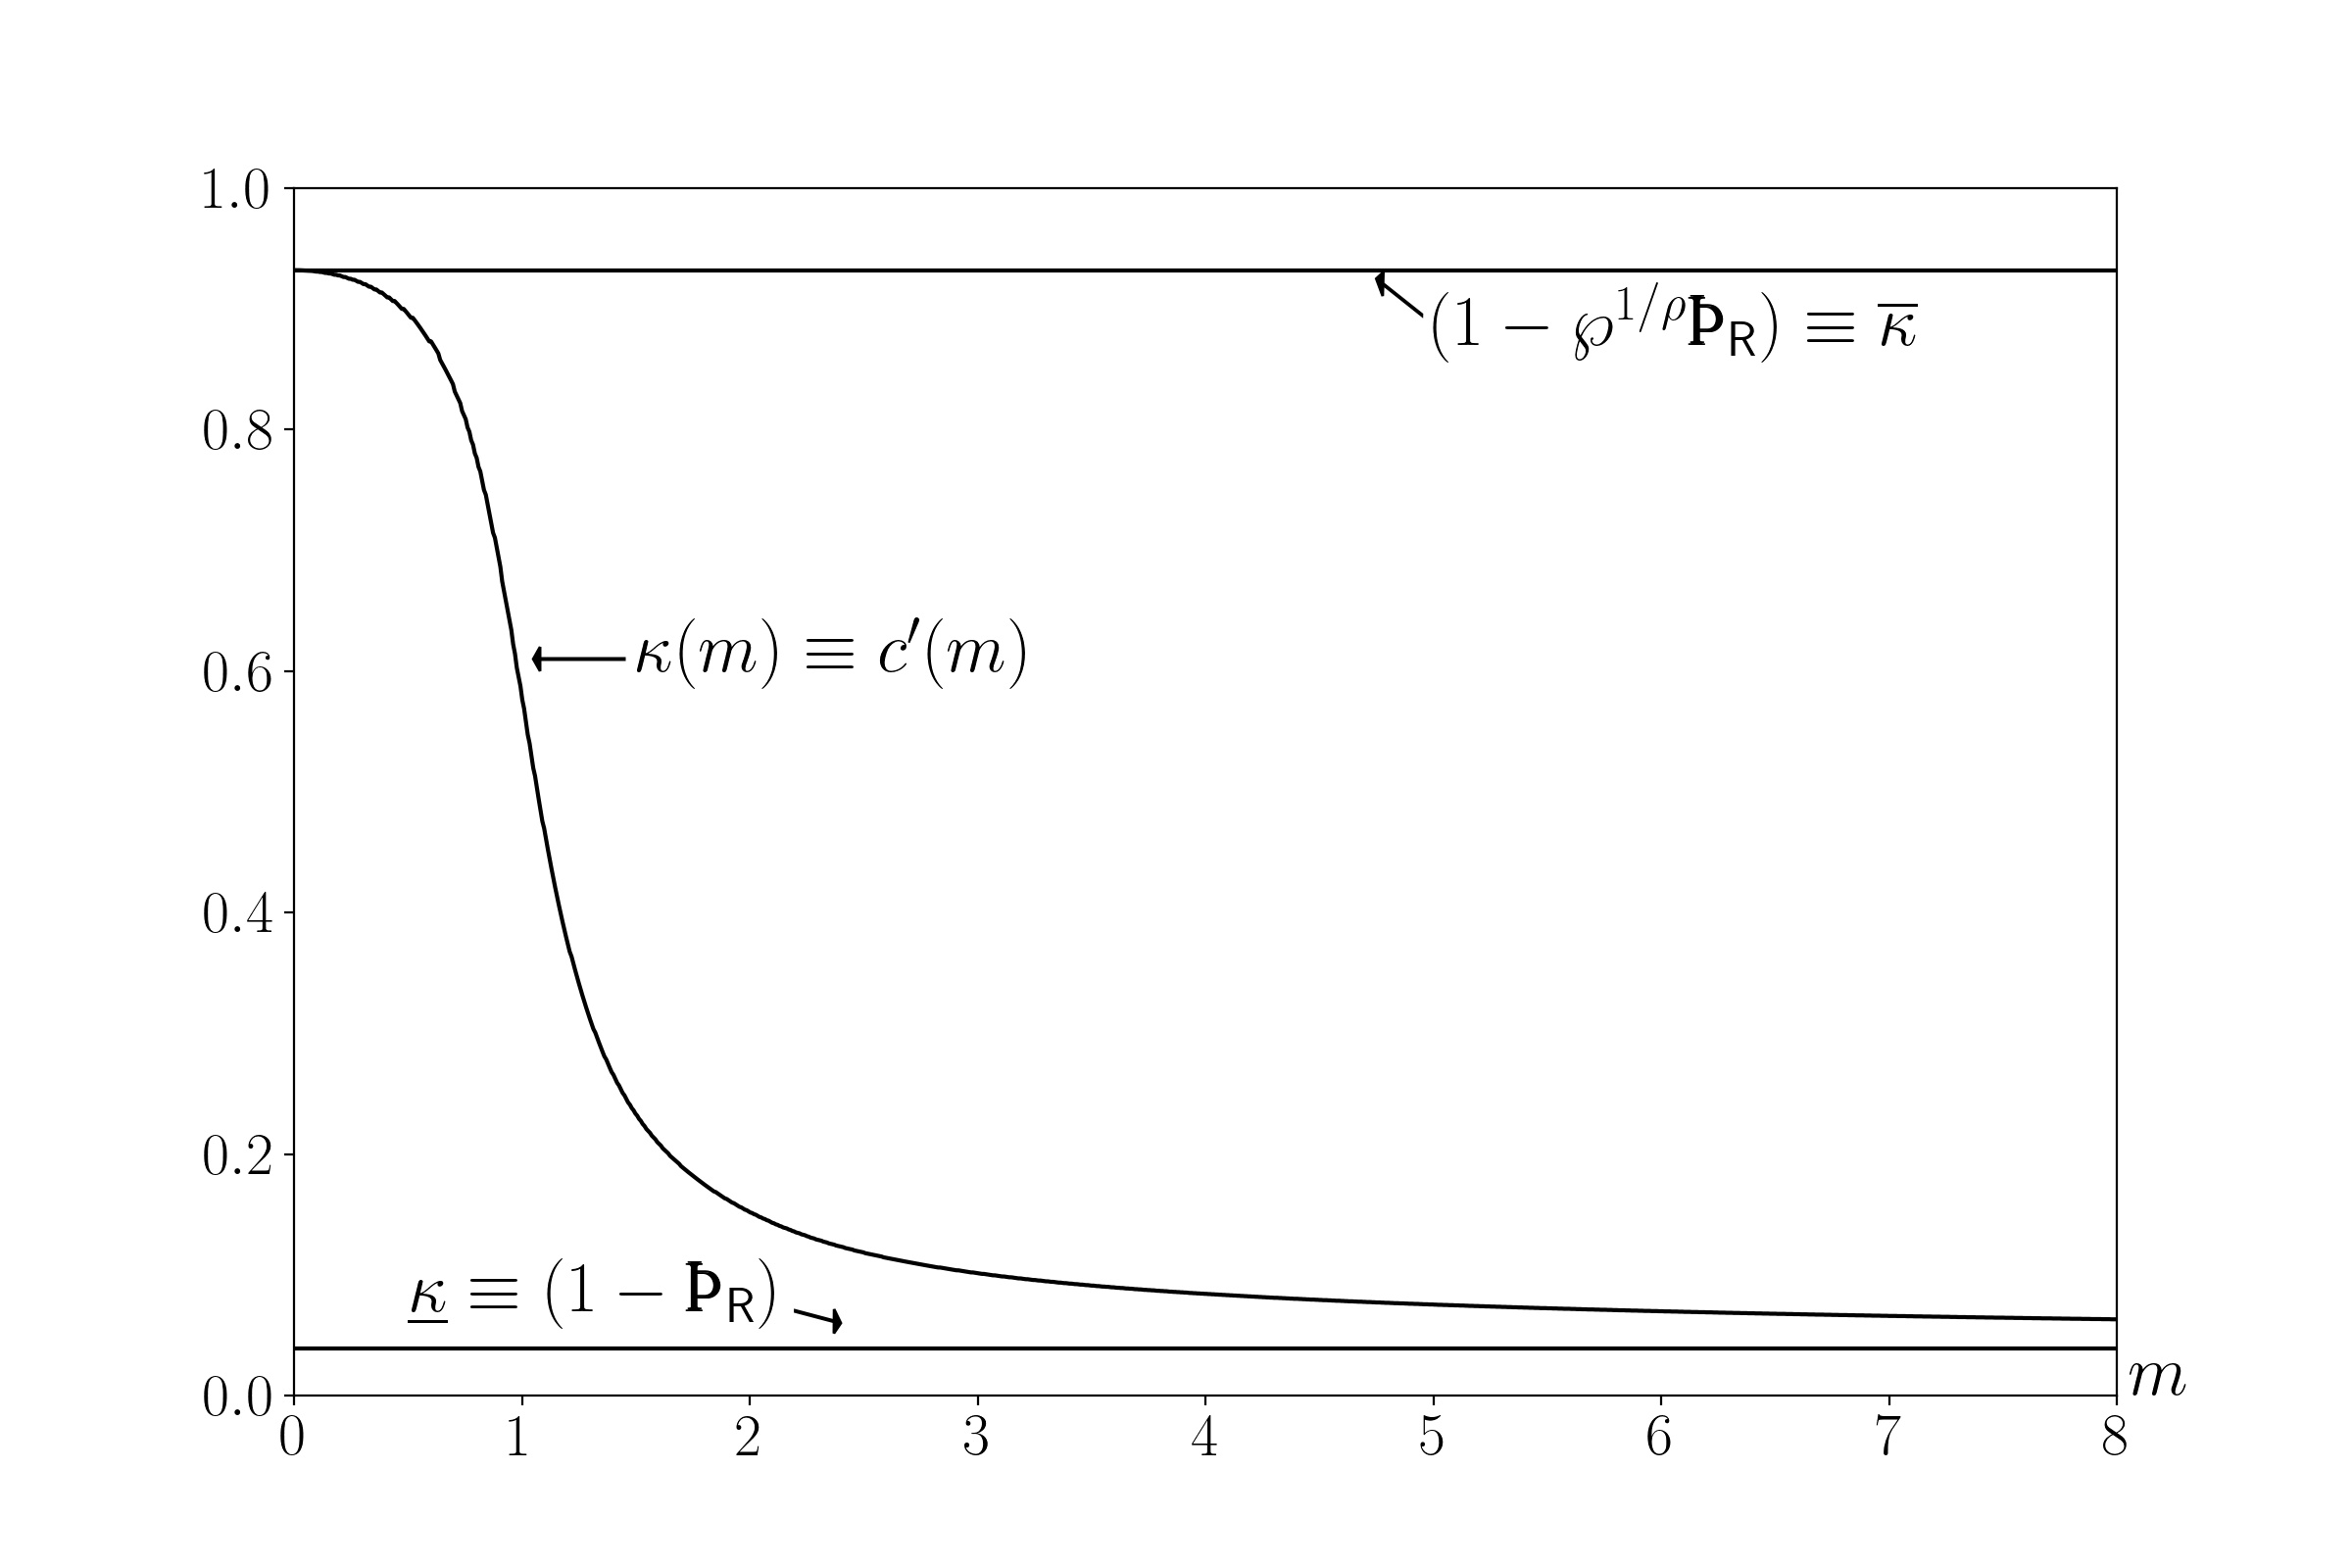
\includegraphics[width=6in]{\FigDir/MPCLimits}}
\caption{Limiting MPC's}
\label{fig:mpclimits}
\end{figure}
} % Web - no

\hypertarget{cFuncBounds}{}
\begin{figure}
\centering
\subfigure[\large Bounds]{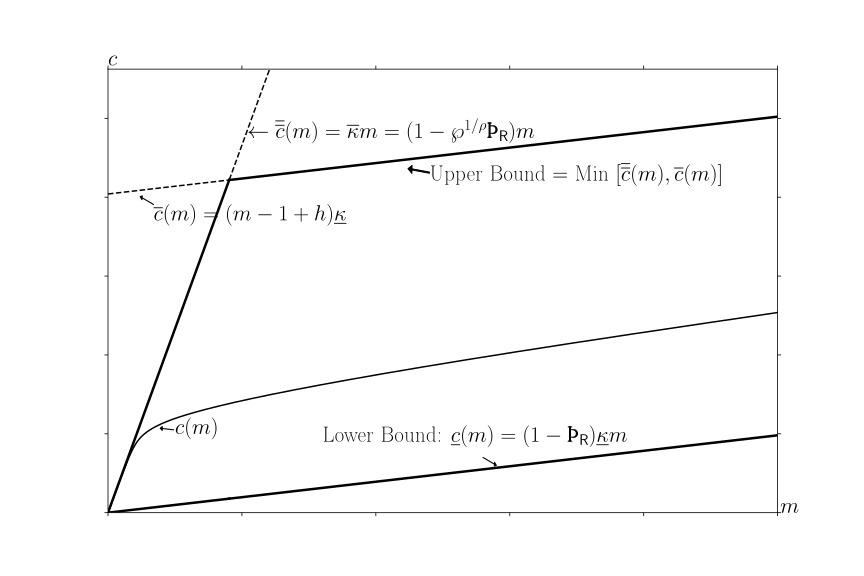
\includegraphics[width=6in]{\FigDir/cFuncBounds}}
\subfigure[\large Target $\mNrm$]{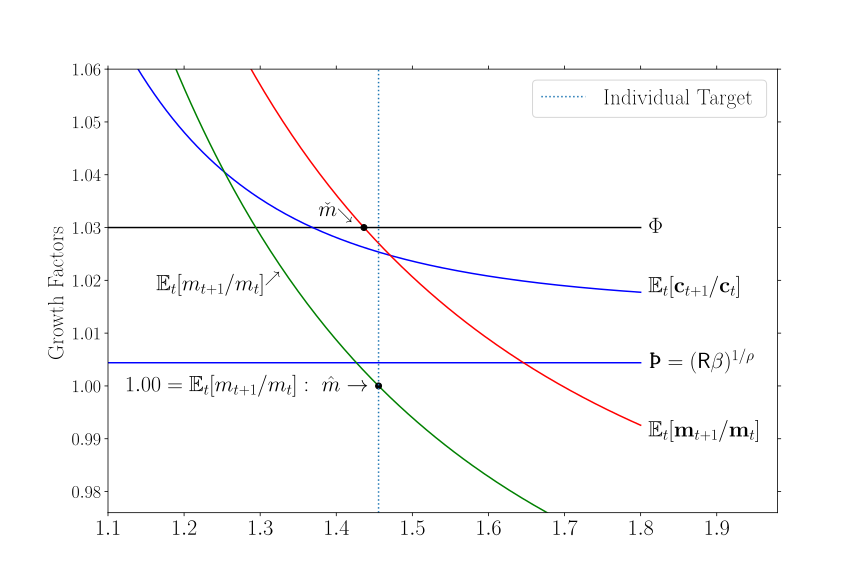
\includegraphics[width=6in]{\FigDir/cNrmTargetFig}}
\caption{The Consumption Function}
\label{fig:cFuncBounds}
\end{figure}

\hypertarget{PFGICHoldsFHWCFailsRICFails}{}
\begin{figure}
\centerline{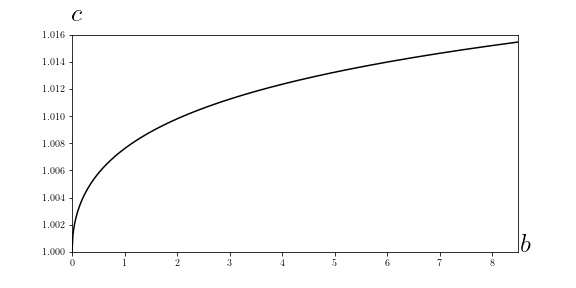
\includegraphics[width=6in]{Figures/PFGICHoldsFHWCFailsRICFails}}
\caption{Appendix: Nondegenerate $\cFunc$ Function with \cncl{FHWC} and \cncl{RIC}}
\label{fig:PFGICHoldsFHWCFailsRICFails}
\end{figure}



\end{document}
% Local Variables:
% eval: (setq TeX-command-list  (assq-delete-all (car (assoc "BibTeX" TeX-command-list)) TeX-command-list))
% eval: (setq TeX-command-list  (assq-delete-all (car (assoc "BibTeX" TeX-command-list)) TeX-command-list))
% eval: (setq TeX-command-list  (assq-delete-all (car (assoc "BibTeX" TeX-command-list)) TeX-command-list))
% eval: (setq TeX-command-list  (assq-delete-all (car (assoc "BibTeX" TeX-command-list)) TeX-command-list))
% eval: (setq TeX-command-list  (assq-delete-all (car (assoc "Biber"  TeX-command-list)) TeX-command-list))
% eval: (add-to-list 'TeX-command-list '("BibTeX" "bibtex ../LaTeX/%s" TeX-run-BibTeX nil t                                                                              :help "Run BibTeX") t)
% eval: (add-to-list 'TeX-command-list '("BibTeX" "bibtex ../LaTeX/%s" TeX-run-BibTeX nil (plain-tex-mode latex-mode doctex-mode ams-tex-mode texinfo-mode context-mode) :help "Run BibTeX") t)
% tex-bibtex-command: "bibtex ../LaTeX/*"
% TeX-PDF-mode: t
% TeX-file-line-error: t
% TeX-debug-warnings: t
% LaTeX-command-style: (("" "%(PDF)%(latex) %(file-line-error) %(extraopts) -output-directory=../LaTeX %S%(PDFout)"))
% TeX-source-correlate-mode: t
% TeX-parse-self: t
% eval: (cond ((string-equal system-type "darwin") (progn (setq TeX-view-program-list '(("Skim" "/Applications/Skim.app/Contents/SharedSupport/displayline -b %n ../LaTeX/%o %b"))))))
% eval: (cond ((string-equal system-type "gnu/linux") (progn (setq TeX-view-program-list '(("Evince" "evince --page-index=%(outpage) ../LaTeX/%o"))))))
% eval: (cond ((string-equal system-type "gnu/linux") (progn (setq TeX-view-program-selection '((output-pdf "Evince"))))))
% TeX-parse-all-errors: t
% End:
